\documentclass[a4paper,oneside,12pt]{extreport}

\usepackage{mmap}
\usepackage[T2A]{fontenc}
\usepackage[utf8]{inputenc}
\usepackage[english,russian]{babel}


% Текст отчёта следует печатать, соблюдая следующие размеры полей:
% левое — 30 мм, правое — 15 мм, верхнее и нижнее — 20 мм.
\usepackage[left=20mm, right=15mm, top=15mm, bottom=15mm]{geometry}

% \setlength{\parindent}{1.25cm} % Абзацный отступ

\usepackage{setspace}
%\onehalfspacing % Полуторный интервал

\frenchspacing % Равномерные пробелы
\usepackage{indentfirst} % Красная строка

\usepackage{microtype}
\sloppy

\usepackage{titlesec}
\titlespacing*{\chapter}{0pt}{-30pt}{8pt}
\titlespacing*{\section}{\parindent}{*4}{*4}
\titlespacing*{\subsection}{\parindent}{*4}{*4}
\titleformat{\chapter}{\LARGE\bfseries}{\thechapter}{20pt}{\LARGE\bfseries}
\titleformat{\section}{\Large\bfseries}{\thesection}{40pt}{\Large\bfseries}

\usepackage{graphicx}
\usepackage{caption}

\usepackage[unicode,pdftex]{hyperref}
\hypersetup{hidelinks}

%% title begin
\usepackage{wrapfig}

\makeatletter
	\def\vhrulefill#1{\leavevmode\leaders\hrule\@height#1\hfill \kern\z@}
\makeatother
%% title end

%% begin code
\usepackage{listings}
\usepackage{xcolor}

\lstset{
	basicstyle=\footnotesize\ttfamily,
	breakatwhitespace=true,
	breaklines=true,
	commentstyle=\color{gray},
	frame=single,
	keywordstyle=\color{blue},
	stringstyle=\color{red},
	tabsize=8
}

\lstdefinestyle{lispinline}{
	frame=none,
	language=Lisp
}

\newcommand{\code}[1]{\texttt{#1}}
%% end code

%% begin theorem
\usepackage{amsthm}

\makeatletter
\newtheoremstyle{indented}
	{}% measure of space to leave above the theorem
	{}% measure of space to leave below the theorem
	{}% name of font to use in the body of the theorem
	{\parindent}% measure of space to indent
	{\bfseries}% name of head font
	{.}% punctuation between head and body
	{ }% space after theorem head; " " = normal interword space
	{}% header specification (empty for default)
\makeatother

\theoremstyle{indented}

\newtheorem{definition}{Определение}[section]
\newtheorem{example}{Пример}[section]
\newtheorem{theorem}{Теорема}[section]
\newtheorem{task}{Задание}

\makeatletter
\DeclareRobustCommand\bfseriesitshape{%
	\not@math@alphabet\itshapebfseries\relax
	\fontseries\bfdefault
	\fontshape\itdefault
	\selectfont
}
\makeatother

\DeclareTextFontCommand{\textbfit}{\bfseriesitshape}
\DeclareTextFontCommand{\define}{\bfseriesitshape}
%% end theorem

%% begin columns
\usepackage{etoolbox,refcount}
\usepackage{multicol}

\newcounter{countitems}
\newcounter{nextitemizecount}
\newcommand{\setupcountitems}{%
	\stepcounter{nextitemizecount}%
	\setcounter{countitems}{0}%
	\preto\item{\stepcounter{countitems}}%
}
\makeatletter
\newcommand{\computecountitems}{%
	\edef\@currentlabel{\number\c@countitems}%
	\label{countitems@\number\numexpr\value{nextitemizecount}-1\relax}%
}
\newcommand{\nextitemizecount}{%
	\getrefnumber{countitems@\number\c@nextitemizecount}%
}
\newcommand{\previtemizecount}{%
	\getrefnumber{countitems@\number\numexpr\value{nextitemizecount}-1\relax}%
}
\makeatother
\newenvironment{AutoMultiColItemize}{%
	\ifnumcomp{\nextitemizecount}{>}{3}{\begin{multicols}{2}}{}%
		\setupcountitems\begin{itemize}}%
		{\end{itemize}%
		\unskip\computecountitems\ifnumcomp{\previtemizecount}{>}{3}{\end{multicols}}{}}
\makeatother
\newenvironment{AutoMultiColEnumerate}{%
	\ifnumcomp{\nextitemizecount}{>}{3}{\begin{multicols}{2}}{}%
		\setupcountitems\begin{enumerate}}%
		{\end{enumerate}%
		\unskip\computecountitems\ifnumcomp{\previtemizecount}{>}{3}{\end{multicols}}{}}
%% end columns



\begin{document}

\begin{titlepage}
	\noindent\begin{minipage}{0.05\textwidth}
		
\includegraphics[scale=0.3]{inc/bmstu.png}
	\end{minipage}
	\hfill
	\begin{minipage}{0.85\textwidth}\raggedleft
		\begin{center}
			\fontsize{12pt}{0.3\baselineskip}\selectfont \textbf{Министерство науки и высшего образования Российской Федерации \\ Федеральное государственное бюджетное образовательное учреждение \\ высшего образования \\ <<Московский государственный технический университет \\ имени Н.Э. Баумана \\ (национальный исследовательский университет)>> \\ (МГТУ им. Н.Э. Баумана)}
		\end{center}
	\end{minipage}

	\begin{center}
		\fontsize{12pt}{0.1\baselineskip}\selectfont
		\noindent\makebox[\linewidth]{\rule{\textwidth}{4pt}} \makebox[\linewidth]{\rule{\textwidth}{1pt}}
	\end{center}

	\begin{flushleft}
		\fontsize{12pt}{0.8\baselineskip}\selectfont 
		
		ФАКУЛЬТЕТ \uline{<<\textbf{Информатика и системы управления}>> \hfill}

		КАФЕДРА \uline{\mbox{\hspace{4mm}} <<\textbf{Программное обеспечение ЭВМ и информационные технологии}>> \hfill}
	\end{flushleft}

	\vfill

	\begin{center}
		\fontsize{20pt}{\baselineskip}\selectfont

		\uline{\textbf{ОТЧЁТ ПО ПРОИЗВОДСТВЕННОЙ ПРАКТИКЕ}}
	\end{center}
	
	\vfill
	
	\begin{flushleft}
		\fontsize{12pt}{0.7\baselineskip}\selectfont

		Студент \uline{\mbox{\hspace{44mm}} Богаченко Артём Евгеньевич \hfill}
		
		Группа \uline{\mbox{\hspace{64mm}} ИУ7-65Б \hfill}
		
		Тип практики \uline{\mbox{\hspace{44mm}} Производственная \hfill}
		
		Название предприятия \uline{\mbox{\hspace{26mm}} ООО~<<Эррайвал РУС>> \hfill}
	\end{flushleft}	

	\vfill

	\begin{table}[h!]
		\fontsize{12pt}{0.7\baselineskip}\selectfont

		\begin{signstabular}[0.55]{p{7.25cm} >{\centering\arraybackslash}p{4cm} >{\centering\arraybackslash}p{4cm}}
		Студент & \uline{\mbox{\hspace*{4cm}}} & \uline{\hfill \textbf{Богаченко А. Е.} \hfill} \\
		& \scriptsize \textit{подпись, дата} & \scriptsize \textit{фамилия, и.о.}
		\end{signstabular}
	
		\vspace{\baselineskip}

		\begin{signstabular}[0.55]{p{7.25cm} >{\centering\arraybackslash}p{4cm} >{\centering\arraybackslash}p{4cm}}
			Руководитель практики & \uline{\mbox{\hspace*{4cm}}} & \uline{\hfill \textbf{Толпинская Н. Б.} \hfill} \\
			\mbox{\hspace*{1cm}} \scriptsize (от университета) & \scriptsize \textit{подпись, дата} & \scriptsize \textit{фамилия, и.о.}
		\end{signstabular}

		\vspace{\baselineskip}
		
		\begin{signstabular}[0.55]{p{7.25cm} >{\centering\arraybackslash}p{4cm} >{\centering\arraybackslash}p{4cm}}
			Руководитель практики & \uline{\mbox{\hspace*{4cm}}} & \uline{\hfill \textbf{Холодная Т. Ю.} \hfill} \\
			\mbox{\hspace*{1cm}} \scriptsize (от предприятия) & \scriptsize \textit{подпись, дата} & \scriptsize \textit{фамилия, и.о.}
		\end{signstabular}
	
		\vspace{\baselineskip}
		
		\begin{signstabular}[0.55]{p{7.25cm} >{\centering\arraybackslash}p{4cm} >{\centering\arraybackslash}p{4cm}}
			Оценка~~\uline{\hfill}
		\end{signstabular} 
	 
	\end{table}

	\vfill

	\begin{center}
		\normalsize \textit{\the\year~г.}
	\end{center}
\end{titlepage}

\section*{Практическая часть}

\begin{task}
    Разработать программу, позволяющую:
    \begin{enumerate}
        \item сформировать список из элементов числового списка, больших заданного значения;
        \item сформировать список из элементов, стоящих на нечетных позициях исходного списка (нумерация от 0);
        \item удалить заданный элемент из списка (один или все вхождения);
        \item преобразовать список в множество (можно использовать ранее разработанные процедуры).
    \end{enumerate}

    Список из элементов числового списка, больших заданного значения:
    \begin{lstlisting}[language=Prolog]
DOMAINS
    list = integer*.

PREDICATES
    f(list, integer, list).

CLAUSES
    f([H|T], Elem, [H|Res]) :-
        H > Elem, !,
        f(T, Elem, Res).
        
    f([_|T], Elem, Res) :-
        f(T, Elem, Res), !.
    
    f([], _, []) :- !.

GOAL
    f([4, 5,1, 4, 6], 3, Result).
    \end{lstlisting}

    \begin{figure}[ht!]
        \centering{
            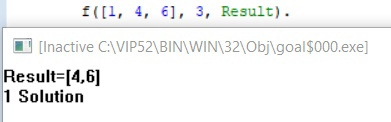
\includegraphics[width=0.8\textwidth]{img/1.jpg}
            \caption{Результат работы первого задания}}
        \end{figure}

    \newpage

    Список из элементов, стоящих на нечетных позициях исходного списка (нумерация от 0):
    \begin{lstlisting}[language=Prolog]
DOMAINS
    list = integer*.
    
    PREDICATES
    odd(list, list).
    
CLAUSES
    odd([_,H|T], [H|Res]) :- odd(T, Res).
    odd([_], []) :- !.
    odd([],[]) :- !.
    
GOAL
    odd([0, 1, 2, 3, 4, 5, 7], Result).
    \end{lstlisting}

    \begin{figure}[ht!]
    \centering{
        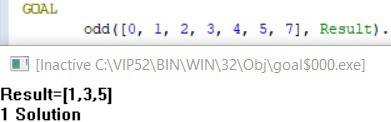
\includegraphics[width=0.8\textwidth]{img/2.jpg}
        \caption{Результат работы второго задания}}
    \end{figure}


    Удаление заданного элемента из списка и преобразование списка в множество:
    \begin{lstlisting}[language=Prolog]
DOMAINS
    list = integer*.

PREDICATES
    del(integer, list, list).
    createSet(list, list).

CLAUSES
    del(Elem, [H|T], [H|Res]) :- 
        H <> Elem, !,
        del(Elem, T, Res).
        
    del(Elem, [_|T], Res) :-
        del(Elem, T, Res), !.
    
    del(_, [], []) :- !.
    
    
    createSet([H|T], [H|Res]) :-
        del(H, T, Tmp),
        createSet(Tmp, Res).
    createSet([], []).

GOAL
    del(3, [4, 3, 1, 2, 3], Result).
    % createSet([1, 2, 3, 4, 5, 6, 1, 2, 3, 4, 5, 3, 2, 6], Result).
    \end{lstlisting}
        
    \begin{figure}[ht!]
    \centering{
        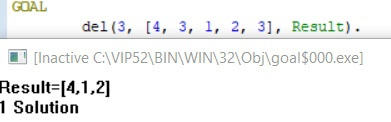
\includegraphics[width=0.8\textwidth]{img/3.jpg}
        \caption{Результат работы третьего задания}}
    \end{figure}

    \begin{figure}[ht!]
    \centering{
        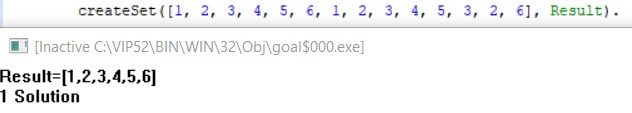
\includegraphics[width=0.8\textwidth]{img/4.jpg}
        \caption{Результат работы четвертого задания}}
    \end{figure}

\end{task}

\newpage


\end{document}